

% This document was generated by the publish-function
% from GNU Octave 4.2.1



\documentclass[10pt]{article}
\usepackage{listings}
\usepackage{mathtools}
\usepackage{amssymb}
\usepackage{graphicx}
\usepackage{hyperref}
\usepackage{xcolor}
\usepackage{titlesec}
\usepackage[utf8]{inputenc}
\usepackage[T1]{fontenc}
\usepackage{lmodern}


\lstset{
language=Octave,
numbers=none,
frame=single,
tabsize=2,
showstringspaces=false,
breaklines=true}


\titleformat*{\section}{\Huge\bfseries}
\titleformat*{\subsection}{\large\bfseries}
\renewcommand{\contentsname}{\Large\bfseries Contents}
\setlength{\parindent}{0pt}

\begin{document}

{\Huge\section*{test}}

\tableofcontents
\vspace*{4em}

\begin{lstlisting}
%Home Work9
\end{lstlisting}
\begin{lstlisting}[language={},xleftmargin=5pt,frame=none]

\end{lstlisting}


\phantomsection
\addcontentsline{toc}{section}{15307130224 GuoZhen She}
\subsection*{15307130224 GuoZhen She}

\begin{lstlisting}
quantity = 10;


% Initialization
A = rand(quantity);
A = A'*A
b = randn(quantity,1)


% Gradient descent
[x, norm_rk, k] = GD(A,b);
figure(1)
plot(norm_rk(1,1:k));
xlabel("k");
ylabel("norm(r_k)");
title("Normal Gradient");


% Gradient descent
a = 3
[x, norm_rk, k] = CG(A,b);
figure(2)
plot(norm_rk(1,1:k));
xlabel("k");
ylabel("norm(r_k)");
title("Conjugate Gradient");
\end{lstlisting}
\begin{lstlisting}[language={},xleftmargin=5pt,frame=none]
A =
 Columns 1 through 8:
   3.8867   2.3049   3.0317   2.3764   3.3421   2.0709   2.8745   2.6193
   2.3049   2.6436   2.1365   1.9379   3.5222   2.7645   2.1944   2.0504
   3.0317   2.1365   3.9213   2.4505   3.1409   2.5427   2.4963   3.2624
   2.3764   1.9379   2.4505   2.5906   2.6666   2.1218   2.0093   2.0931
   3.3421   3.5222   3.1409   2.6666   5.1758   3.3803   3.2108   2.8492
   2.0709   2.7645   2.5427   2.1218   3.3803   3.5573   2.2995   2.6835
   2.8745   2.1944   2.4963   2.0093   3.2108   2.2995   2.7558   2.5780
   2.6193   2.0504   3.2624   2.0931   2.8492   2.6835   2.5780   3.3437
   2.7603   2.0540   2.1704   1.8423   2.8814   2.1811   2.3729   2.2792
   2.0224   1.7989   2.2451   2.3840   2.6553   1.8938   1.8230   2.0634
 Columns 9 and 10:
   2.7603   2.0224
   2.0540   1.7989
   2.1704   2.2451
   1.8423   2.3840
   2.8814   2.6553
   2.1811   1.8938
   2.3729   1.8230
   2.2792   2.0634
   2.7069   1.6986
   1.6986   2.8650
b =
  -2.31343
   0.24417
  -0.81010
   2.19298
   1.39457
   0.77246
   1.62016
   0.27664
   2.54034
  -1.04158
a =  3

\end{lstlisting}
\begin{figure}[!ht]
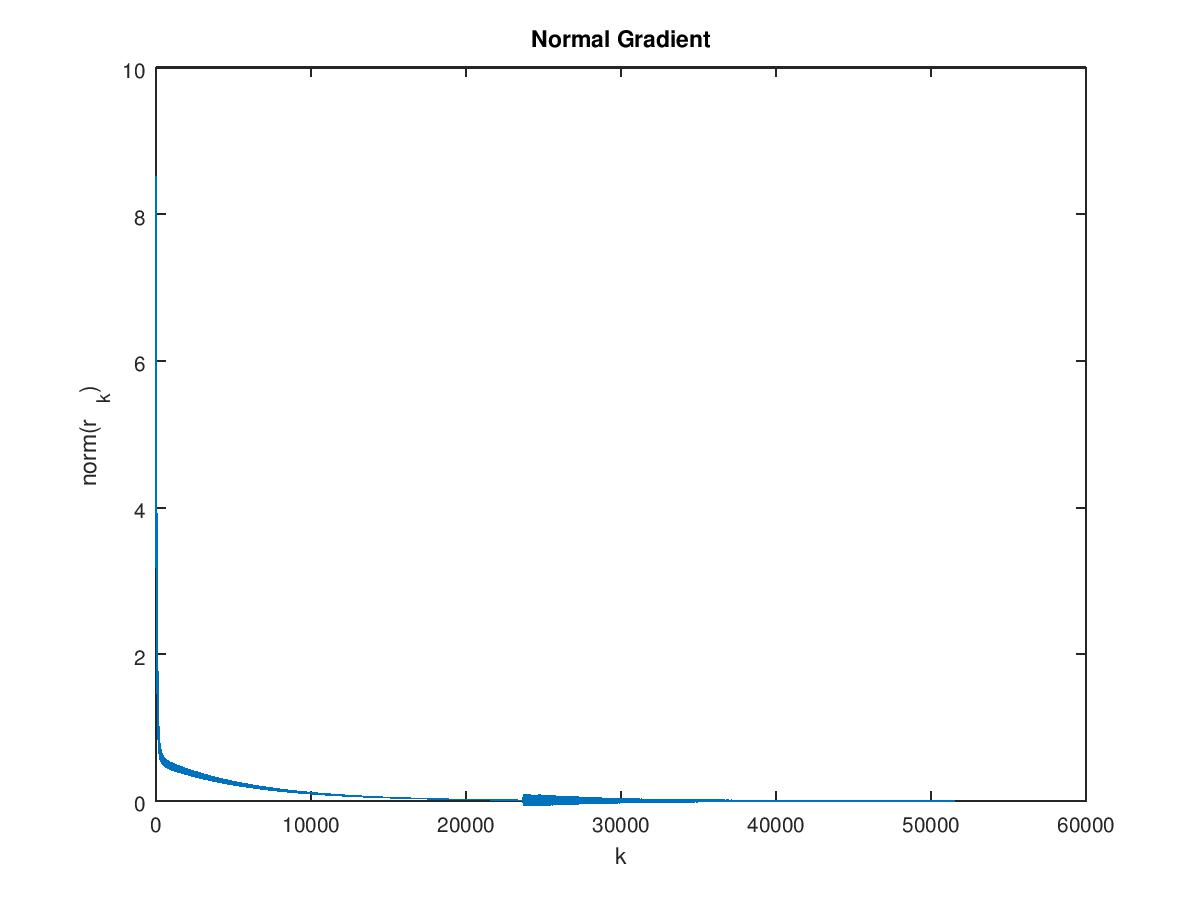
\includegraphics[width=\textwidth]{test-1.jpg}
\end{figure}
\begin{figure}[!ht]
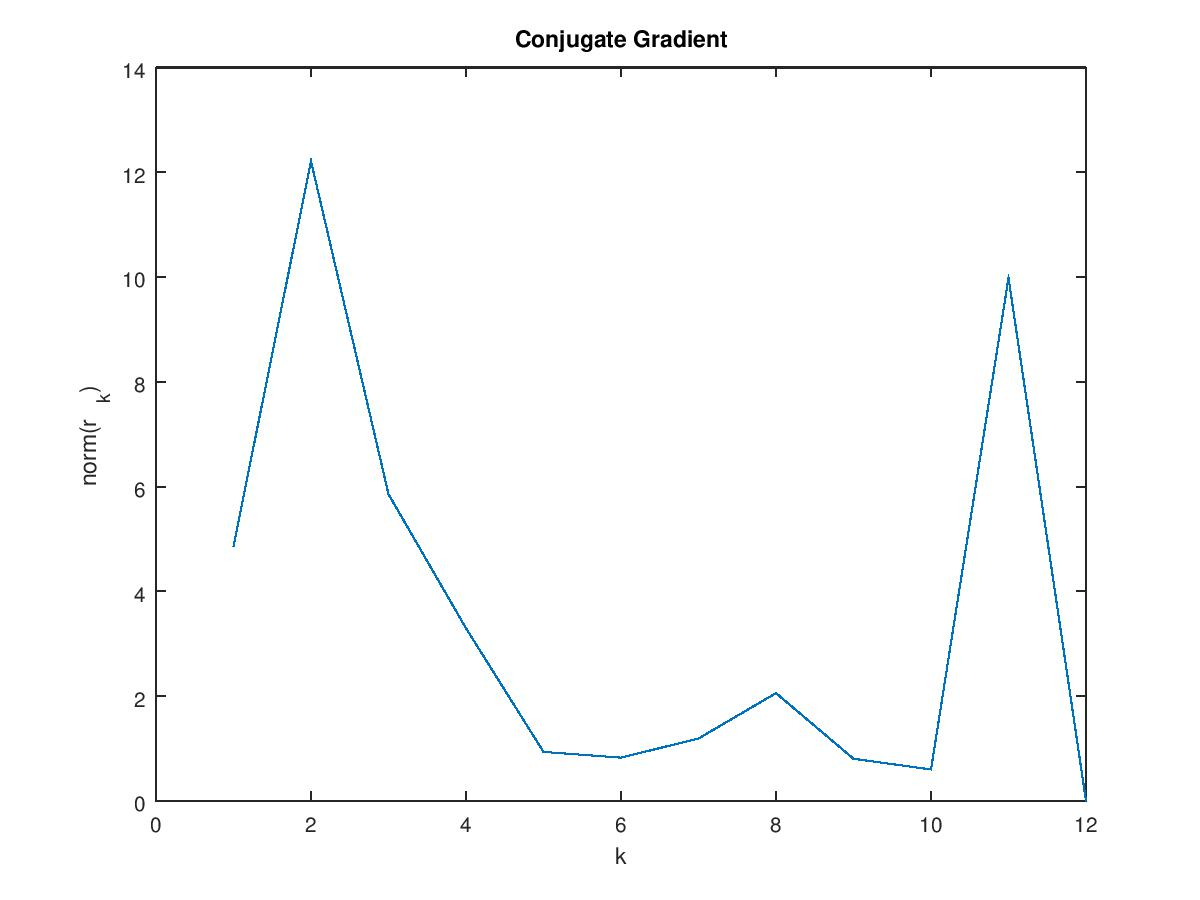
\includegraphics[width=\textwidth]{test-2.jpg}
\end{figure}


\end{document}
